%++++++++++++++++++++++++++++++++++++++++
% Don't modify this section unless you know what you're doing!
\documentclass[letterpaper,12pt]{article}
\usepackage{tabularx} % extra features for tabular environment
\usepackage{amsmath}  % improve math presentation
\usepackage{graphicx} % takes care of graphic including machinery
\usepackage[margin=1in,letterpaper]{geometry} % decreases margins
\usepackage{cite} % takes care of citations
\usepackage[final]{hyperref} % adds hyper links inside the generated pdf file
\usepackage[toc,page]{appendix}
\usepackage{listings}

\hypersetup{
	colorlinks=true,       % false: boxed links; true: colored links
	linkcolor=blue,        % color of internal links
	citecolor=blue,        % color of links to bibliography
	filecolor=magenta,     % color of file links
	urlcolor=blue         
}
%++++++++++++++++++++++++++++++++++++++++


\begin{document}

\title{M4S18A2 Machine Learning - Coursework 2  }
\author{Omar Haque}
\date{\today}
\maketitle

\section*{Introduction}
This report has 3 sections. In the first, I implement a K-means clustering algorithm, and a Gaussian Mixture Model under the Expectation-Maximisation framework. I use these algorithms to create a program which automatically segments and counts the number of cells in a medical image. In the second part I explore the role of bias in modern AI applications. In the third section, I implement a Hidden-Markov Model in order to create a predictive trading model for Ethereum prices.



\section*{Question 1}

Here is the implementation for the K-means algorithm

\begin{lstlisting}[language=python]
def k_means_clustering(X_cleaned,K=10,maxiter=200):

    # get dimensions of data
    n = X_cleaned.shape[0]
    dim = X_cleaned.shape[1]
    
    ## initialise centroids randomly
    random.seed(1)
    centroids = X_cleaned[random.sample(range(n),K),:]
    
    # initialise convergence criteria
    converged = False
    
    for i in range(maxiter):
        
        # bookkeeping, simply keep track of the old centroids
        old_centroids = centroids
        
        # data assignment step
        data_clustering = get_closest_cluster(X_cleaned, centroids,K)
        # centroids update step
        centroids = update_centroids(X_cleaned, data_clustering,K)
        
        if (np.allclose(centroids,old_centroids,rtol=1e-3)):
            print("converged at iteration " + str((i+1)))
            converged = True
            break
        
    if (not converged):
        print("Warning, clusters did not converge.")
    
    return centroids, data_clustering
\end{lstlisting}

\section{Theory}

Here give a brief summary of the physical effect of interest and provide
necessary equations. Here is how you insert an equation. According to
references~\cite{melissinos, Cyr, Wiki} the dependence of interest is given
by
\begin{equation} \label{eq:aperp} % the label is used to reference the equation
u(\lambda,T)=\frac{8\pi hc\lambda^{-5}}{e^{hc/\lambda kT}-1},
\end{equation}
where T is temperature in Kelvin, c is the speed of light, etc. Don't forget to
explain what each variable means the first time that you introduce it.


\section{Procedures}

Give a schematic of the experimental setup(s) used in the experiment (see
figure~\ref{fig:samplesetup}). Give the description of  abbreviations
either in the figure caption or in the text. Write a description of what is
going on. 

\begin{figure}[ht] 
        % read manual to see what [ht] means and for other possible options
        \centering 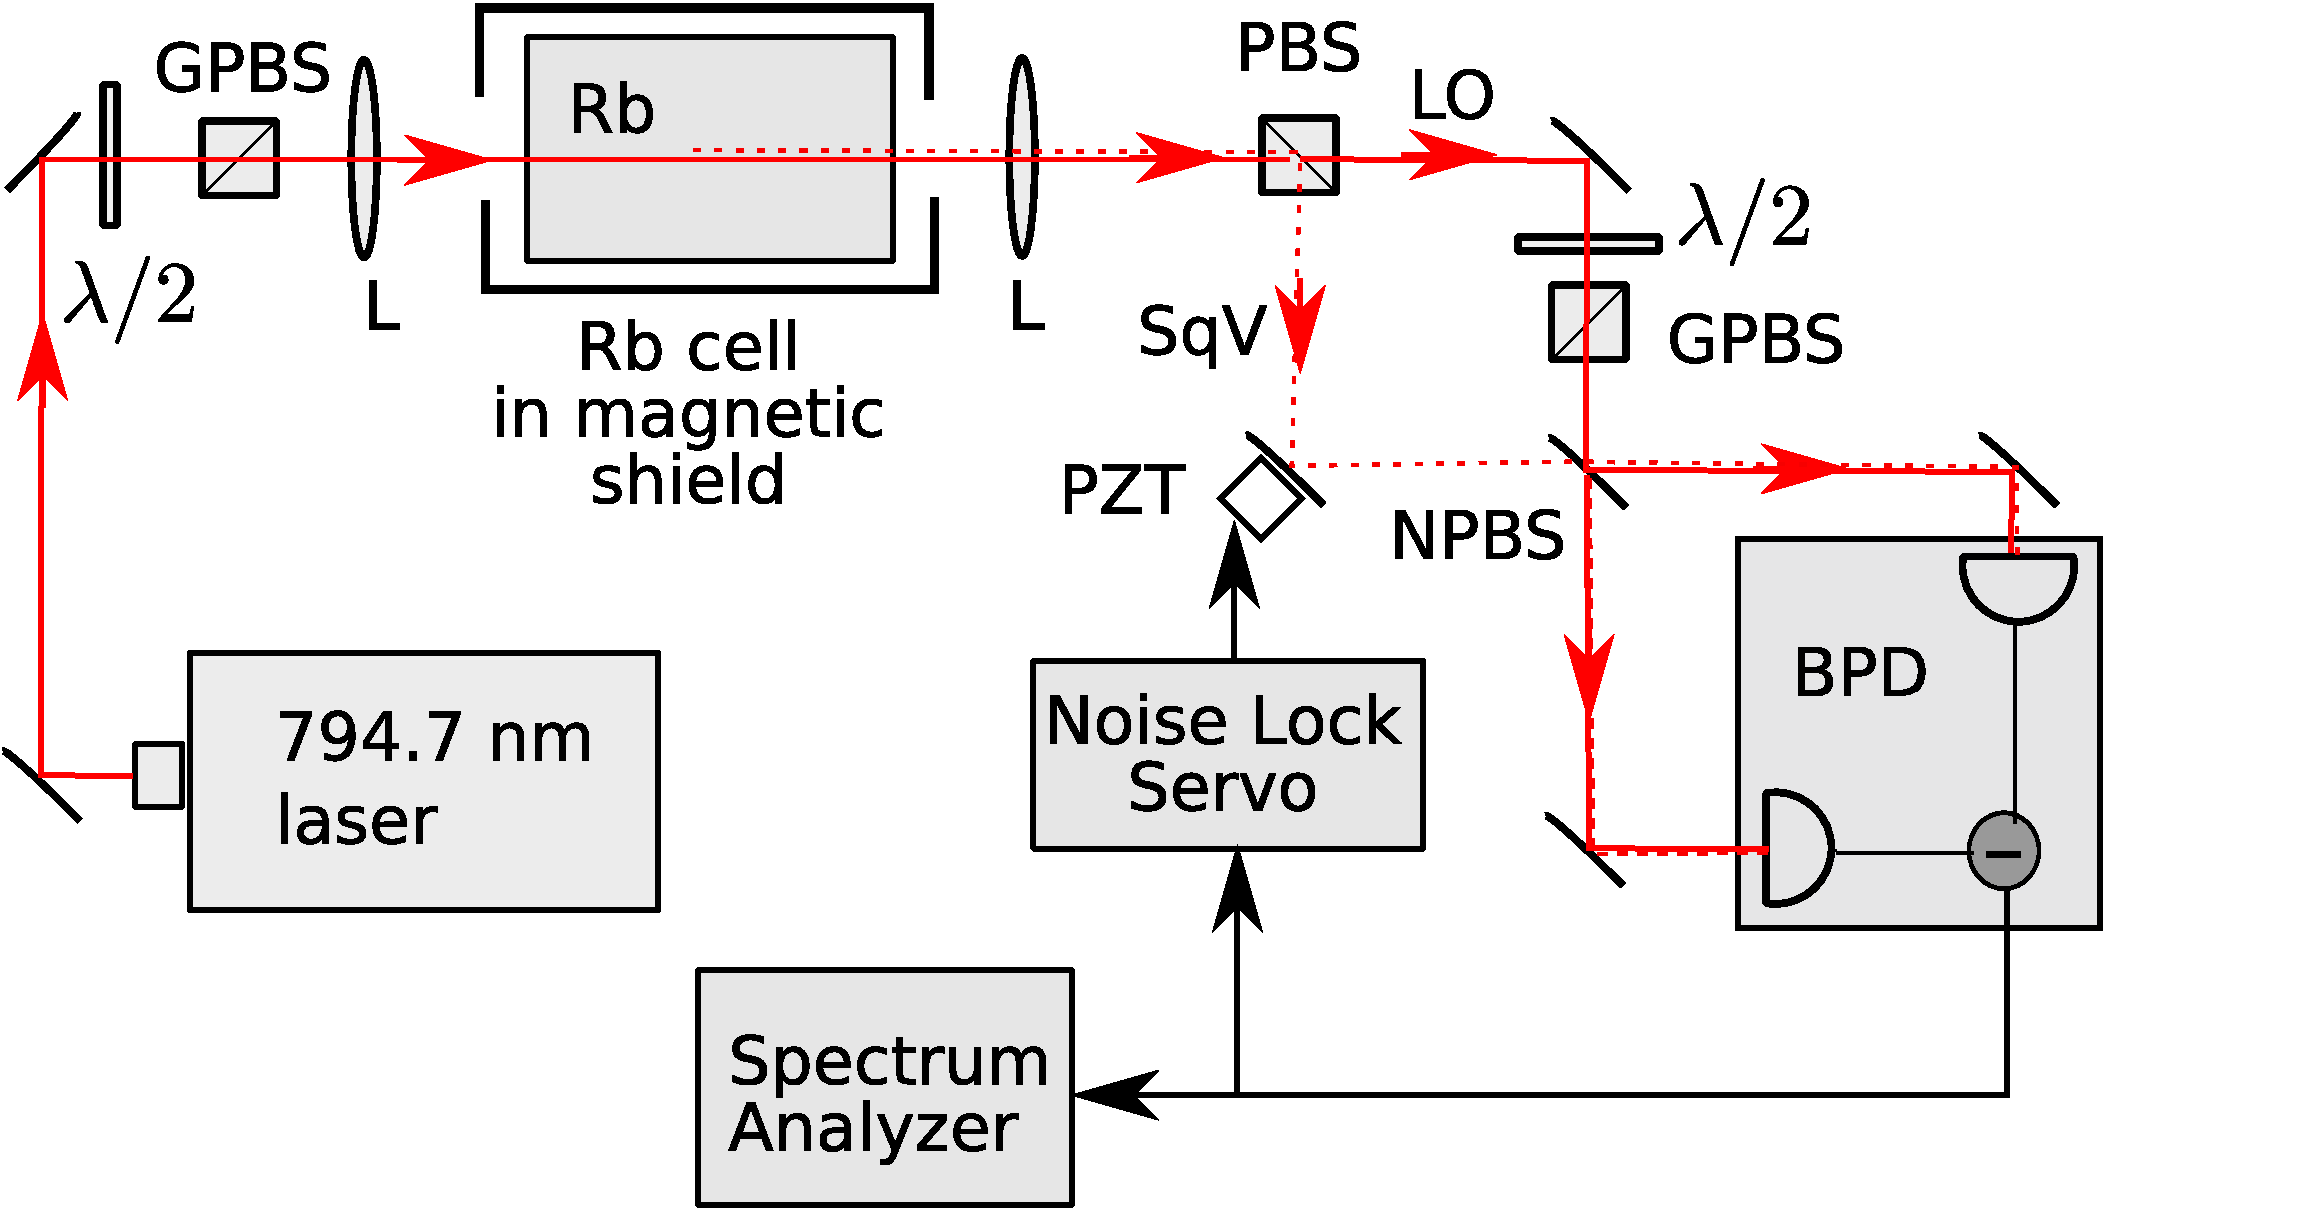
\includegraphics[width=0.8\columnwidth]{sr_setup}
        % note that in above figure file name, "sr_setup",
        % the file extension is missing. LaTeX is smart enough to find
        % apropriate one (i.e. pdf, png, etc.)
        % You can add this extention yourself as it seen below
        % both notations are correct but above has more flexibility
        %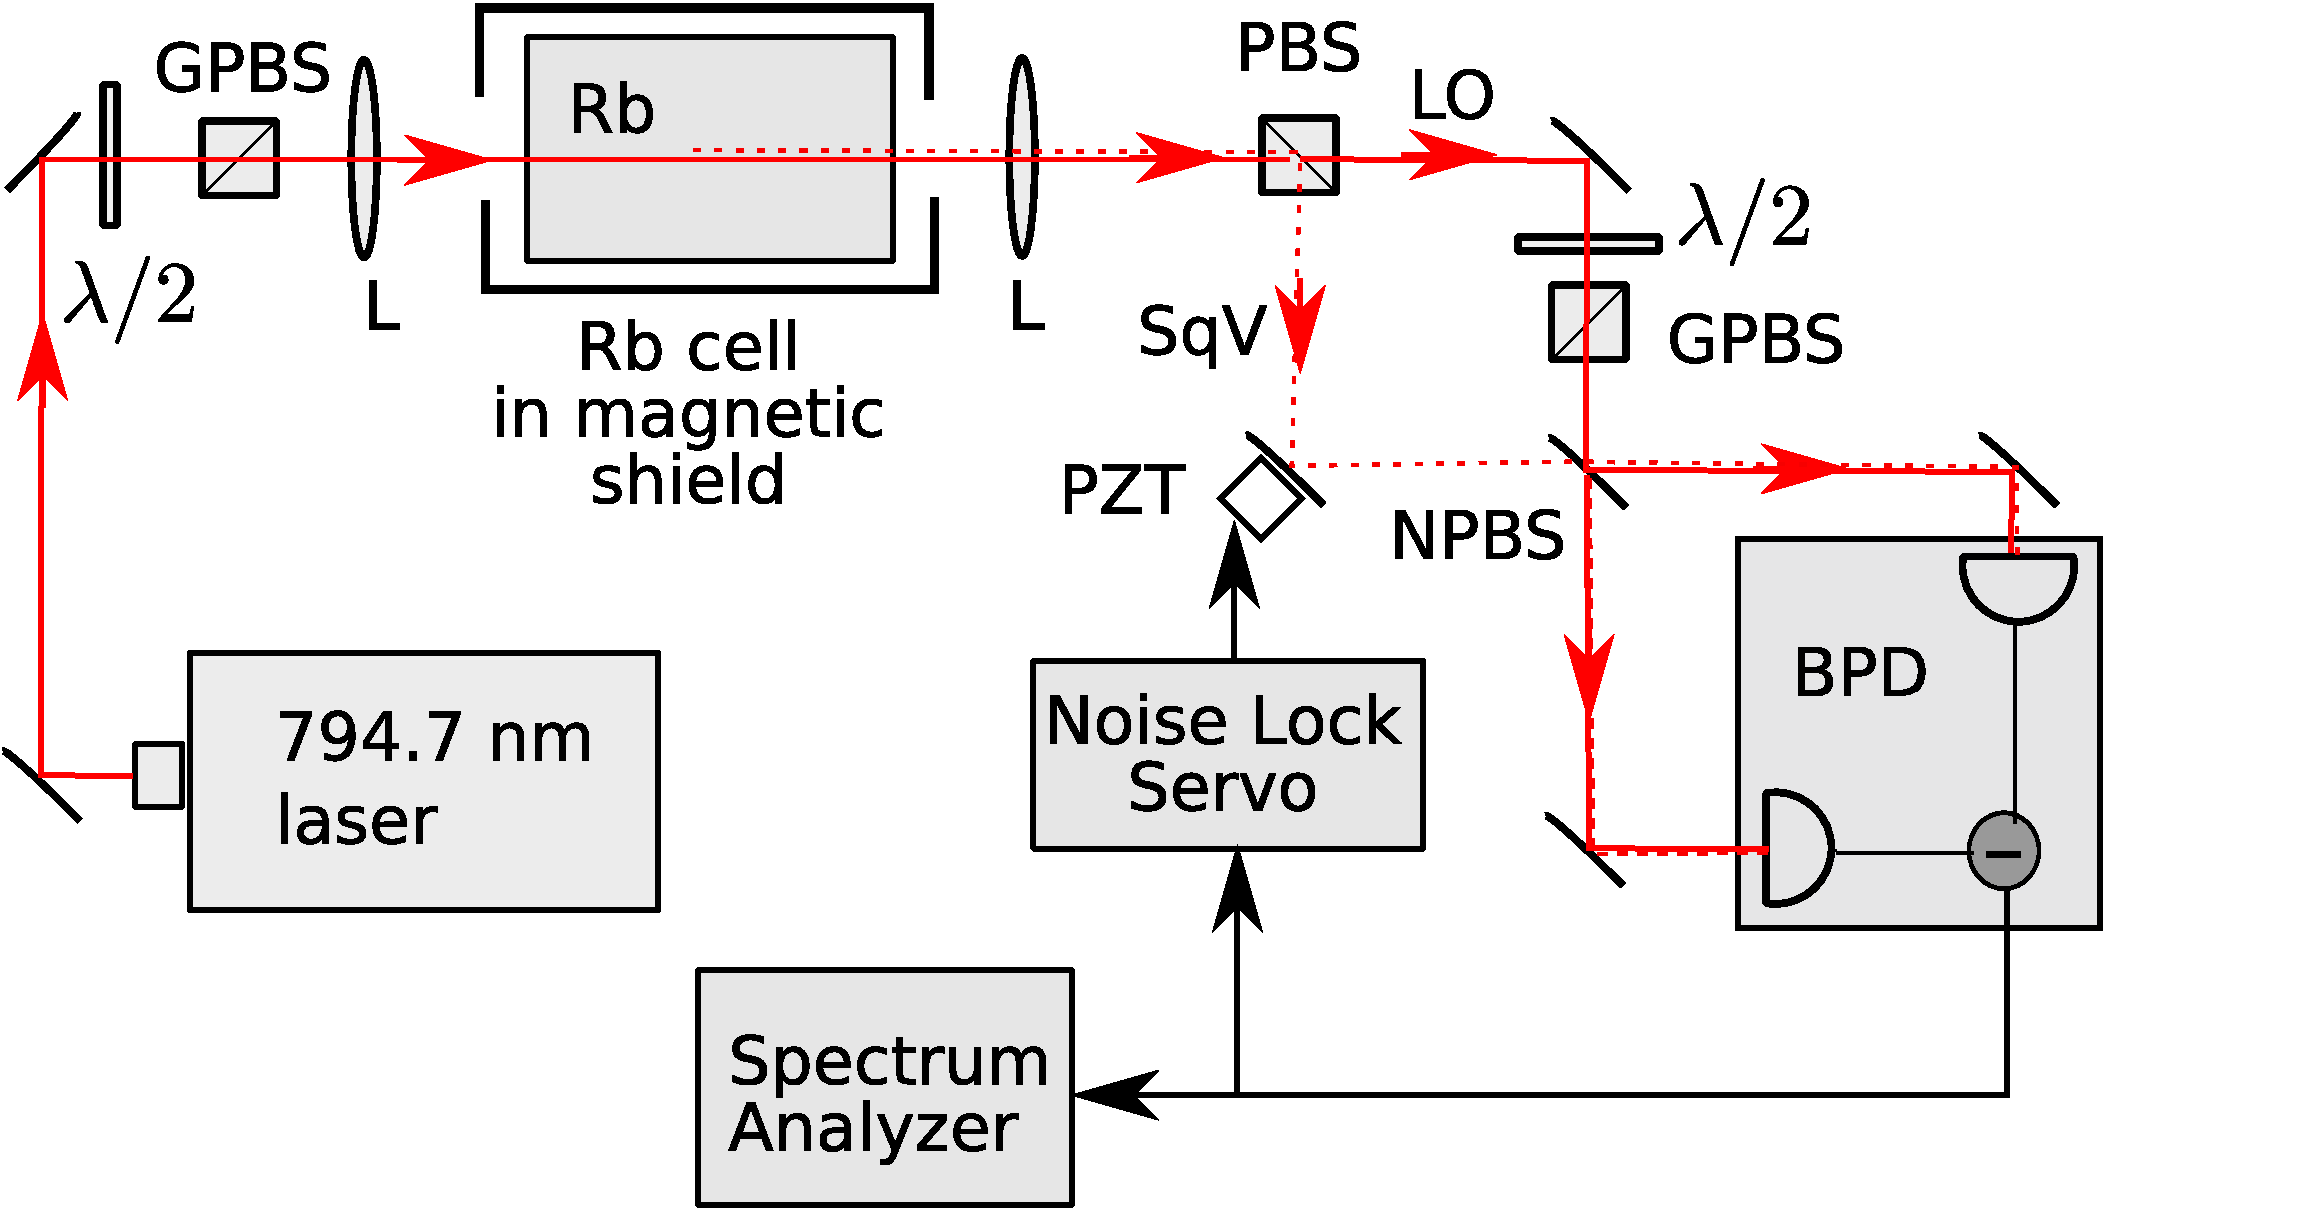
\includegraphics[width=1.0\columnwidth]{sr_setup.pdf}
        \caption{
                \label{fig:samplesetup} % spaces are big no-no withing labels
                % things like fig: are optional in the label but it helps
                % to orient yourself when you have multiple figures,
                % equations and tables
                Every figure MUST have a caption.
        }
\end{figure}

Don't forget to list all important steps in your experimental procedure!

Use active voice either in past or present through all the report and be
consistent with it:
The laser light comes  from to ... and eventually arrived to the
balanced photodiode as seen in the figure~\ref{fig:samplesetup}.

Sentences in the past voice while correct are generally considered hard to read
in large numbers. The laser light was directed to ..., wave plates were set
to ... etc.


\section{Analysis}

In this section you will need to show your experimental results. Use tables and
graphs when it is possible. Table~\ref{tbl:bins} is an example.

\begin{table}[ht]
\begin{center}
\caption{Every table needs a caption.}
\label{tbl:bins} % spaces are big no-no withing labels
\begin{tabular}{|cc|} 
\hline
\multicolumn{1}{|c}{$x$ (m)} & \multicolumn{1}{c|}{$V$ (V)} \\
\hline
0.0044151 &   0.0030871 \\
0.0021633 &   0.0021343 \\
0.0003600 &   0.0018642 \\
0.0023831 &   0.0013287 \\
\hline
\end{tabular}
\end{center}
\end{table}

Analysis of equation~\ref{eq:aperp} shows ...

Note: this section can be integrated with the previous one as long as you
address the issue. Here explain how you determine uncertainties for different
measured values. Suppose that in the experiment you make a series of
measurements of a resistance of the wire $R$ for different applied voltages
$V$, then you calculate the temperature from the resistance using a known
equation and make a plot  temperature vs. voltage squared. Again suppose that
this dependence is expected to be linear~\cite{Cyr}, and the proportionality coefficient
is extracted from the graph. Then what you need to explain is that for the
resistance and the voltage the uncertainties are instrumental (since each
measurements in done only once), and they are $\dots$. Then give an equation
for calculating the uncertainty of the temperature from the resistance
uncertainty. Finally explain how the uncertainty of the slop of the graph was
found (computer fitting, graphical method, \emph{etc}.)

If in the process of data analysis you found any noticeable systematic
error(s), you have to explain them in this section of the report.

It is also recommended to plot the data graphically to efficiently illustrate
any points of discussion. For example, it is easy to conclude that the
experiment and theory match each other rather well if you look at
Fig.~\ref{fig:samplesetup} and Fig.~\ref{fig:exp_plots}.

\begin{figure}[ht] 
  \centering
      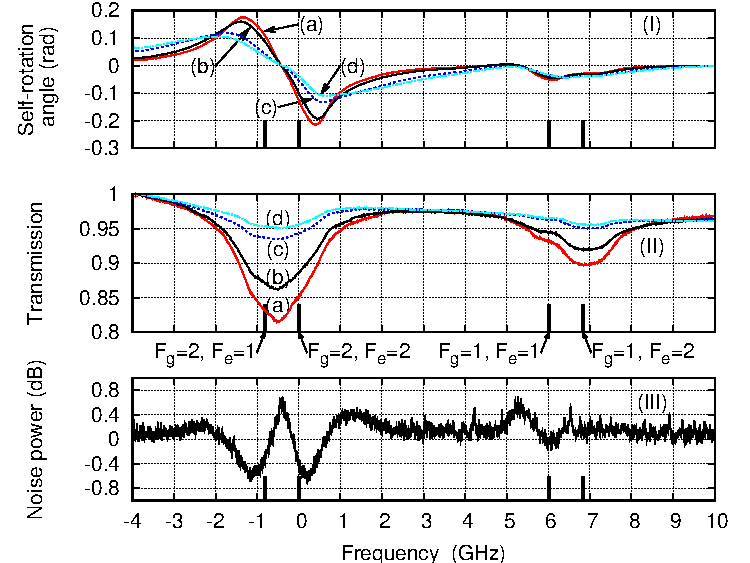
\includegraphics[width=0.5\columnwidth]{sr_squeezing_vs_detuning}

% some figures do not need to be too wide
        \caption{
                \label{fig:exp_plots}  
                Every plot must have axes labeled.
        }
\end{figure}


\section{Conclusions}
Here you briefly summarize your findings.

%++++++++++++++++++++++++++++++++++++++++
% References section will be created automatically 
% with inclusion of "thebibliography" environment
% as it shown below. See text starting with line
% \begin{thebibliography}{99}
% Note: with this approach it is YOUR responsibility to put them in order
% of appearance.

\begin{thebibliography}{99}

\bibitem{melissinos}
A.~C. Melissinos and J. Napolitano, \textit{Experiments in Modern Physics},
(Academic Press, New York, 2003).

\bibitem{Cyr}
N.\ Cyr, M.\ T$\hat{e}$tu, and M.\ Breton,
% "All-optical microwave frequency standard: a proposal,"
IEEE Trans.\ Instrum.\ Meas.\ \textbf{42}, 640 (1993).

\bibitem{Wiki} \emph{Expected value},  available at
\texttt{http://en.wikipedia.org/wiki/Expected\_value}.

\end{thebibliography}


\end{document}
